\documentclass[10pt,a4paper]{article}
\usepackage[T1]{fontenc}
\usepackage[utf8]{inputenc}
\usepackage{lmodern}
\usepackage[margin=24mm]{geometry}
\usepackage{amsmath,amssymb,booktabs,array,longtable,graphicx,microtype}
\usepackage{xcolor}
\definecolor{ink}{HTML}{243447}
\usepackage[colorlinks=true,linkcolor=ink,citecolor=ink,urlcolor=ink]{hyperref}
\usepackage{url}
\makeatletter
\newcommand{\tableinput}[1]{\@@input #1 }
\makeatother
\setlength{\parskip}{3pt}
\setlength{\parindent}{1em}
\setlength{\emergencystretch}{2em}
\widowpenalty=10000
\clubpenalty=10000
\renewcommand{\arraystretch}{1.15}
\title{Cognitive Atlas: Reconstructing Geographic Geometry\\from Repeated Multilingual LLM Distance Judgments}
\author{}
\date{8 September 2026\\\small Exploratory research draft; not peer reviewed}
\begin{document}
\maketitle
\begin{abstract}
A language model can answer individual geographic questions accurately without its answers defining a coherent world. We present a file-based experimental pipeline that preserves repeated capital-to-capital distance judgments, evaluates them against WGS84 geodesics, and reconstructs their implied geometry using Euclidean and spherical embeddings. An initial three-model comparison covers 50 capitals and 1,225 unordered pairs, with ten requested responses per pair. A matched five-language Gemini 3.5 Flash experiment collects a further 61,250 completed samples using English, French, Spanish, Arabic, and Mandarin Chinese instructions. Among 1,223 pairs with ten valid responses in every language, all ten language comparisons exhibit median-distance disagreement exceeding a within-pair label-permutation baseline (Holm-adjusted Monte Carlo $p=0.004$). Similar overall accuracy can nevertheless conceal substantial changes in individual estimates. An exploratory local-language analysis finds that Spanish instructions reduce mean single-response absolute error on pairs involving six Spanish-associated capitals by 17.4 km, or 7.0\%, relative to English. The corresponding advantage over other pairs is 24.5 km; both contrasts have adjusted bootstrap $p=0.0008$. No comparable positive local advantage is established for the other three languages. These findings are conditional on the selected capitals, one translation per language, one collection period, and independence of API samples. The reconstructed geometry is a description of observable judgments, not a direct measurement of hidden neural representations.
\end{abstract}

\section{Introduction and scope}
What geographic world is implied by a model's answers when every pair of places is queried repeatedly? This question separates factual accuracy from the geometric compatibility of the answers. It also separates the stability of repeated responses from their correctness: an identical answer can be consistently wrong.

Geographic structure in language is an established research topic. Louwerse and Zwaan recovered geographic relationships from distributional text statistics \cite{louwerse}. Bhandari et al. used prompting and multidimensional scaling to study LLM geospatial knowledge \cite{bhandari}. Karimi and Janowicz examined distance-estimation challenges, including variation across English and Persian prompts \cite{karimi}. Our application of MDS to prompted geography is therefore not claimed as a first. The practical contribution here is an auditable repeated-sampling implementation, matched multilingual numeric-response protocols, spherical reconstruction, and explicit separation of global judgment differences from geographically localized accuracy gains.

Internal-representation studies answer a different question. Gurnee and Tegmark used model activations to investigate spatial and temporal representations \cite{gurnee}. We access only API responses. Memorized facts, numerical heuristics, language-conditioned associations, and internal computation can all produce the behavior studied here; this design cannot identify which mechanism is responsible.

The report addresses three questions: (1) do the estimates track actual geography and admit a useful reconstruction; (2) do matched instruction languages produce differences larger than repeated-call variation; and (3) do prompts in a language particularly improve accuracy for capitals associated with that language? All analyses are exploratory. There was no preregistration, and the local-language question was formulated after the global language results had been inspected.

\section{Data and experimental design}
\subsection{Capital sample and reference distances}
The main sample contains 50 purposively selected national capitals across six inhabited continents. It expands an initial 20-capital pilot; it is neither a random sample of countries nor the complete set of sovereign states. Appendix~\ref{app:capitals} lists every included city. Natural Earth populated-place coordinates supply documented reference points, with dataset-specific overrides and capital-selection decisions retained in the repository \cite{naturalearth}. Examples include Pretoria as South Africa's executive capital and Dodoma as Tanzania's capital. A city is represented by one point, so differences between city centers or administrative boundaries remain a source of reference uncertainty.

For each unordered pair $p=(i,j)$, the reference distance $t_p$ is the WGS84 inverse geodesic calculated with GeographicLib \cite{karney}. There are $50\times49/2=1{,}225$ pairs. These geodesics are stored separately from model outputs. They are the real-distance benchmark used throughout, rather than distances measured in a flat map projection.

\subsection{Conditions and sampling}
An English-language model comparison uses Gemini 2.5 Flash-Lite, Gemini 3 Flash Preview, and Gemini 3.5 Flash. Exact API identifiers are preserved in the manifests. Ten separate single-turn requests are scheduled for each pair. All three expanded conditions use temperature 1, top-$p$ 0.95, and a maximum of 128 output tokens. Thinking is disabled with a zero budget for 2.5 Flash-Lite; the other two use the provider's minimal thinking setting. These controls are not equivalent, so the comparison concerns these configurations, not isolated model architecture or scale. No tools, conversation history, or earlier sampled answers are supplied. No generation seed is specified.

The language experiment holds the model at Gemini 3.5 Flash and uses English, French, Spanish, Arabic, and Mandarin Chinese instructions. The city and country strings remain in their canonical English forms. Only instructions are translated; this is not a test of localized place names. The translations are assistant-authored and have not received independent native-speaker validation. The Spanish and Chinese versions, for example, explicitly describe the great-circle distance as the shortest path along Earth's surface; instruction language and particular wording cannot be separated.

Every language uses the same added numeric-format rule: ASCII digits, a period if a decimal separator is needed, and no thousands separators or units. A new English baseline was collected with this rule. The earlier English model-comparison run is not used as the baseline for language inference. Exact prompts are preserved in manifests, response rows, and the supplement \texttt{results/exact-language-prompts.json}.

The five language conditions were collected concurrently during one period on 8 September 2026, starting at approximately 16:56 UTC and finishing at approximately 17:35 UTC. A shared dispatch limit of 2,400 requests per minute and per-condition caps of 900 were configured. Concurrent dispatch reduces simple sequential ordering differences, but it is not randomized assignment of language to time blocks. The API returned the same model-version alias across these conditions; the alias does not establish a frozen weight checkpoint.

\subsection{Quality control and data retention}
The language protocol accepts exactly one positive ASCII decimal number no larger than 20,040 km. Complete raw text and provider payloads are preserved even when parsing fails. Eleven language-study responses exceeded the range threshold and two violated numeric formatting. One transport timeout was retried, yielding 61,251 recorded attempts, 61,250 completed sample slots, and 61,237 valid estimates. Invalid content is terminal and is not replaced by repeated attempts until a plausible answer appears.

All descriptive full-matrix metrics use accepted observations. For matched inferential analyses, we exclude the two pairs lacking ten valid responses in any language: Buenos Aires--Hanoi and Seoul--Moscow. The common subset contains 1,223 pairs and 61,150 valid observations. This is a complete-case analysis, not an outlier filter based on estimated accuracy. Nevertheless, the range rule removes particularly implausible judgments and can make accepted-output accuracy optimistic. Invalid counts are therefore outcomes of the experiment, not disposable records.

\section{Analysis and reconstruction}
\subsection{Repeated observations and accuracy}
For valid responses $x_{p\ell r}$ in pair $p$, language $\ell$, and replicate $r$, we retain all observations and calculate the mean, median, 10\% trimmed mean per tail, Huber location, sample variance and standard deviation, extrema, quartiles, interquartile range, median absolute deviation, and coefficient of variation. Huber fitting uses scale $\max(1.4826\,\mathrm{MAD},1\,\mathrm{km})$. Four aggregate distance matrices are exported; the median is the presentation baseline, not a demonstrated universally optimal estimator.

Writing $m_{p\ell}$ for the median, median-matrix accuracy is
\begin{equation}
 A^{\rm med}_{\ell}=\frac{1}{P}\sum_p |m_{p\ell}-t_p|.
\end{equation}
We also report RMSE, relative error, Pearson, Spearman and Kendall correlations, and three-nearest-neighbor preservation. A symmetric matrix is created from unordered pairs with zero diagonal. Symmetry is imposed by design, not empirically verified.

\subsection{Geometry and alignment}
All 19,600 triples in the 50-capital dataset are checked for triangle-inequality violations. Spectra of the double-centered squared-distance matrix and the cosine angular-distance matrix supply diagnostics of Euclidean and spherical compatibility. Negative eigenvalues are diagnostics, not a proof of a unique latent dimensionality.

Classical MDS forms $B=-\tfrac12 JD^{\circ2}J$, where $J=I-\mathbf{1}\mathbf{1}^{\mathsf T}/N$, and uses its leading nonnegative eigencomponents. Metric and non-metric MDS use four seeded starts, a maximum of 1,000 iterations, and scikit-learn's SMACOF implementation \cite{kruskal,sklearn}. Non-metric MDS fits monotone disparities, so its reported stress cannot be directly ranked against stress computed on kilometer distances. The pipeline fits metric embeddings in dimensions 1 through 10 and computes the same curve for WGS84 distances.

Spherical reconstruction fits unit vectors $u_i\in S^2$ with fixed radius $R=6371.0088$ km, minimizing
\begin{equation}
 \sum_{i<j}\left[R\arccos(u_i^{\mathsf T}u_j)-D_{ij}\right]^2.
\end{equation}
Initialization comes from the eigendecomposition of $\cos(D/R)$, not from actual city coordinates. Four starts are optimized with sparse analytic derivatives. After fitting, a single orthogonal Procrustes transformation aligns the inferred vectors with reference Earth vectors \cite{schonemann}. Rotations and reflections are permitted; individual cities are never moved independently toward their true locations during fitting or alignment. The spherical radius is fixed. Planar fits instead permit translation, rotation/reflection, and one global scale relative to an explicitly equirectangular reference.

Spherical residual stress is
\begin{equation}
 S=\sqrt{\frac{\sum_{i<j}(\widehat D_{ij}-D_{ij})^2}{\sum_{i<j}D_{ij}^2}}.
\end{equation}
Spherical fitting and ellipsoidal ground truth differ slightly even for perfect judgments. Euclidean embeddings also cannot reproduce global great-circle distances exactly merely by using three coordinates: chord distances and arc distances differ.

\subsection{Map deformation}
For display, a Delaunay triangulation connects reference capitals and fixed frame pins in equirectangular coordinates. Each triangle maps continuously to its inferred vertices by an affine transformation. Densified country boundaries are interpolated through the same field. Longitude branches minimize discontinuities near the map seam, and reversed triangles are counted as foldovers. This procedure interpolates a visual surface between inferred capital positions; it does not measure beliefs about coastlines. Continuity does not guarantee topology preservation. The website exposes capital-only reconstructions, actual locations, displacement vectors, uncertainty summaries, raw samples, and selectable experiment layers alongside the warped view.

\subsection{Global language randomization tests}
For each of the ten language comparisons, two statistics are evaluated on the common complete subset: mean absolute median disagreement,
\begin{equation}
 T_{ab}=P^{-1}\sum_p |m_{pa}-m_{pb}|,
\end{equation}
and the absolute difference in median-matrix MAE. Under the strong null that response distributions are exchangeable between the two languages within each fixed pair, the twenty observations are pooled and independently reassigned to groups of ten. Replicate numbers are not treated as paired observations. We generate 4,999 random assignments for each comparison and use $(b+1)/(B+1)$ Monte Carlo tail probabilities \cite{scipyperm}. The disagreement statistic uses an upper tail; the MAE contrast uses its absolute value. Holm adjustment covers all twenty tests \cite{holm}.

These tests quantify departures from a common response distribution conditional on the fixed cities and independence of requests. In particular, the MAE-contrast test is not a general weak-null test of equal expected accuracy under arbitrary unequal response distributions. The resulting $p$ values should not be read as probabilities that a language is superior in all future uses.

\subsection{Exploratory local-language contrasts}
A language-associated pair has at least one endpoint in the following operational groups:
\begin{center}\small
\begin{tabular}{lp{11cm}}\toprule
French & Ottawa, Kinshasa, Paris, Dakar \\
Spanish & Buenos Aires, Santiago, Bogot\'a, Madrid, Mexico City, Lima \\
Arabic & Algiers, Cairo, Rabat, Riyadh \\
Mandarin Chinese & Beijing, Singapore \\
\bottomrule\end{tabular}
\end{center}
The groups use official/co-official national language status and majority Spanish-language use as a transparent proxy, not individual language proficiency. They include multilingual places and do not assert that any city has only one language. French excludes Algeria and Morocco under this operational definition. The distinction between legal status and actual use is substantive \cite{cervantes,oif,singapore}. These group definitions were fixed before examining the local contrasts, but after examining overall language results.

The local analysis evaluates \emph{single-response} accuracy, a different estimand from error of the median. Define $e_{p\ell r}=|x_{p\ell r}-t_p|$ and
\begin{equation}
 g_{p\ell}=\overline e_{p,\mathrm{en}}-\overline e_{p\ell},\quad
 G_{H\ell}=\frac{1}{|H_\ell|}\sum_{p\in H_\ell}g_{p\ell},\quad
 I_\ell=G_{H\ell}-G_{O\ell},
\end{equation}
where $O_\ell$ contains pairs with neither endpoint in the group. Positive $G_H$ means lower error than English on associated pairs; positive $I$ means that benefit is greater than on other pairs. A positive interaction alone would not guarantee an absolute improvement.

We independently resample ten observations within each pair and language for 9,999 bootstrap replicates. Using the mean of absolute errors avoids the nonregular behavior of bootstrap medians with many tied observations. Centered bootstrap deviations are multiplied by $\sqrt{10/9}$ to match the variance estimate from sample variances with nine degrees of freedom. Basic 95\% intervals invert the deviation quantiles; two-sided approximate $p$ values count centered deviations at least as large as the observed contrast. Holm correction covers eight tests: $G_H$ and $I$ for four languages. Intervals are pointwise, not multiplicity-adjusted. Analytic contrast standard errors independently check the bootstrap implementation. No normal distribution for numeric guesses is assumed.

This bootstrap estimates repeated-call uncertainty on a fixed set of pairs. It does not turn shared-city dyads into independent country-level replications and does not estimate uncertainty across new cities, translated phrasings, or collection dates. As a descriptive sensitivity check, we remove each associated capital and all its pairs in turn. These leave-one-capital-out ranges are not confidence intervals or new significance tests.

\section{Results}
\subsection{Geographic signal and model comparison}
The original English 50-capital runs show strong associations with reference geography (Table~\ref{tab:models}). Their Spearman correlations are approximately 0.967 for 2.5 Flash-Lite and 0.998 for both later configurations. A separate city-label permutation audit with 9,999 permutations gives one-sided Monte Carlo $p=0.0001$ for each, relative to random relabeling of a fixed distance matrix. This establishes geographic signal against that baseline; it does not establish normal sampling distributions, absence of systematic errors, or definitive model rankings.

\begin{table}[htbp]\centering\small
\caption{Original English 50-capital conditions. MAE is error of pair medians, using all accepted observations. These prompts precede the matched language-format protocol.}\label{tab:models}
\begin{tabular}{lrrrr}\toprule
Gemini configuration & Valid samples & MAE (km) & Spearman & Sphere stress \\\midrule
\tableinput{generated/model-table.tex}
\bottomrule\end{tabular}
\end{table}

Repeated answers are often discrete and identical. In the original 3.5 Flash run, 154 of 1,225 pairs return the same value all ten times; London--Paris returns 344 km in all ten samples, against a 341.15 km reference. This is incompatible with treating all observations as unrounded continuous Gaussian draws. Ten samples do not establish the distribution's shape or the model's epistemic uncertainty.

\subsection{Language differences without large changes in global geography}
Full-matrix descriptive results appear in Table~\ref{tab:languages}. All five language conditions remain highly correlated with actual distances. Their spherical reconstructions remain recognizable (Figure~\ref{fig:maps}), while their residual errors and capital placements differ. Illustrative deformation should not be mistaken for an independent statistical result.

\begin{table}[htbp]\centering\small
\caption{Matched language conditions, all 1,225 pairs. Each has 12,250 completed sample slots. Triangles is the percentage violating the inequality; MAE uses pair medians.}\label{tab:languages}
\begin{tabular}{lrrrrr}\toprule
Language & Valid & MAE (km) & Spearman & Triangles (\%) & Sphere stress \\\midrule
\tableinput{generated/language-table.tex}
\bottomrule\end{tabular}
\end{table}


\begin{figure}[htbp]\centering
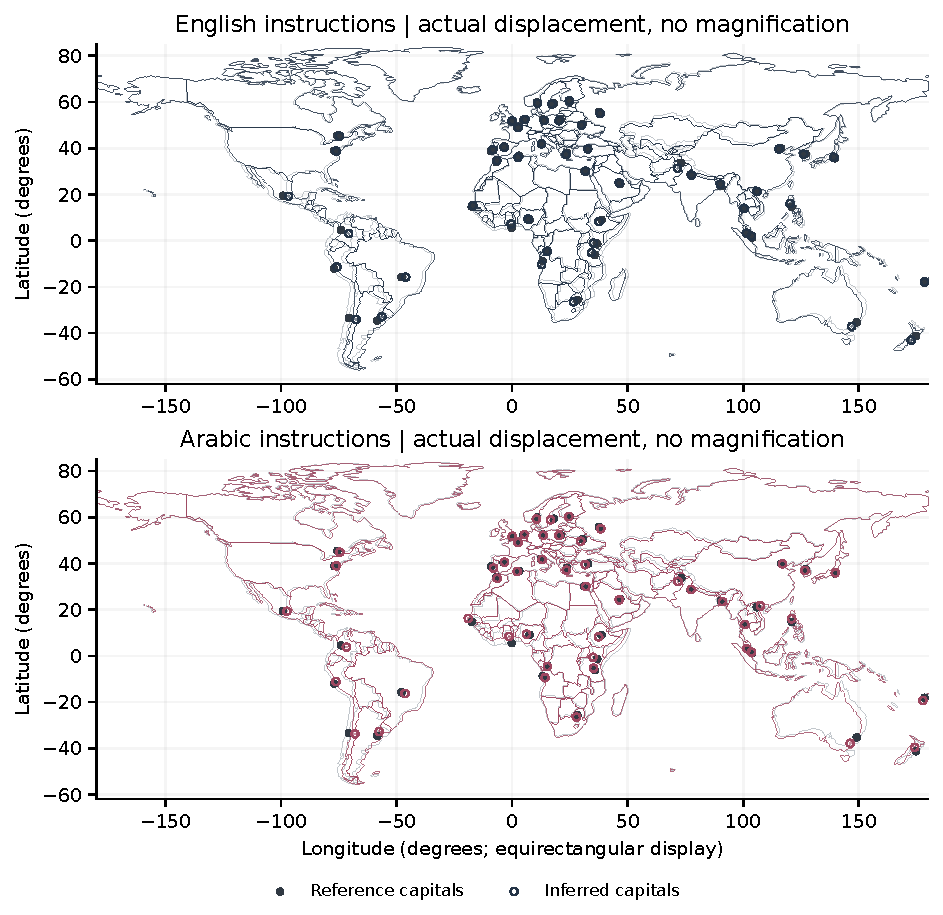
\includegraphics[width=\linewidth]{figures/reconstructed-worlds.pdf}
\caption{Median-based spherical reconstructions for English and Arabic. Gray outlines are reference geography; colored outlines are the stored piecewise-affine deformation. Filled points mark reference capitals and open points mark inferred capitals. Both use the same equirectangular display and actual, unamplified displacement.}\label{fig:maps}
\end{figure}


On the 1,223 complete pairs, every language comparison exceeds its shuffled-label disagreement baseline, with Holm-adjusted $p=0.004$ (Table~\ref{tab:pairwise}). The common value reflects the Monte Carlo resolution and correction, not equality of effect sizes or a measured exact probability. Mandarin versus English shows 122.3 km average disagreement between pair medians, compared with a 55.0 km shuffled-label average, despite only a 0.7 km difference in aggregate median-based MAE. Languages can change the pattern of mistakes while leaving overall accuracy similar.


\begin{figure}[htbp]\centering
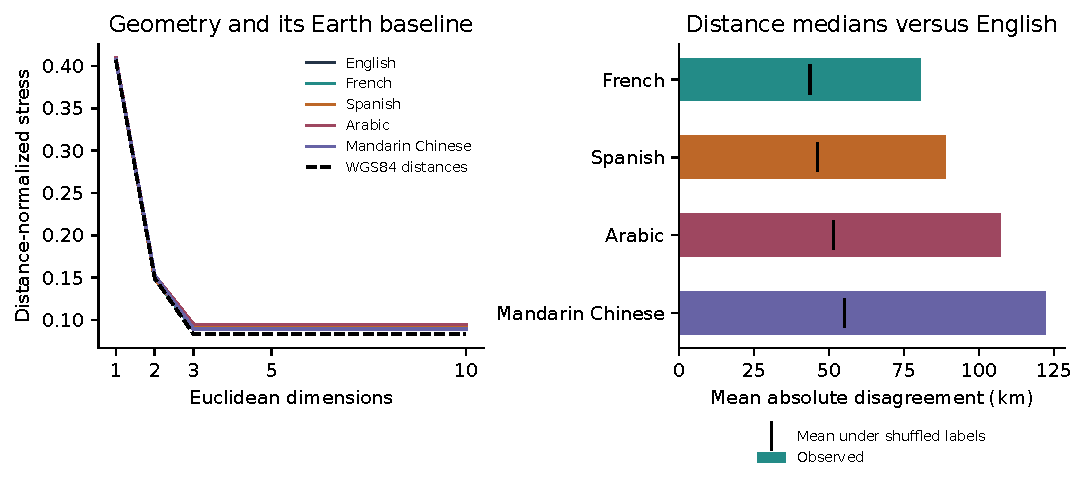
\includegraphics[width=\linewidth]{figures/structure-and-language.pdf}
\caption{Left: metric Euclidean MDS stress by dimension, with the WGS84 baseline. Higher-dimensional residuals should not be attributed wholly to semantic distortion: true Earth arc distances also retain residual Euclidean stress. Slight nonmonotonicity reflects numerical optimization. Right: observed median disagreements with English and the conditional shuffled-label means.}\label{fig:structure}
\end{figure}


\subsection{A Spanish-associated benefit, not a general local-language rule}
Table~\ref{tab:local} and Figure~\ref{fig:local} report the exploratory local contrasts. Spanish has 278 associated complete pairs. Its mean single-response absolute error falls from 249.0 km under English to 231.6 km under Spanish: a 17.4 km reduction (7.0\%; pointwise 95\% interval 9.7--25.1 km). On the 945 other pairs, Spanish instead increases error by 7.2 km. The interaction is therefore $+24.5$ km (95\% interval 16.2--32.8 km). Both adjusted $p$ values are 0.0008.

French does not significantly improve accuracy on its associated pairs: the estimated gain is $-5.0$ km. Its $-11.0$ km interaction is significant within the eight-test family, indicating less benefit there than elsewhere under this classification. Arabic increases error on associated pairs by 22.7 km, with essentially no local interaction. Mandarin increases associated-pair error by 10.5 km, but its local interaction is not significant. A general rule that a model knows a place better when asked in a locally associated language is therefore unsupported.


\begin{table}[htbp]\centering\scriptsize
\caption{Local-language analysis on 1,223 complete pairs. Errors average individual responses, not pair medians. $G_H$ and $I$ are gains in km; positive favors the translated prompt. Adjusted $p$ values use one family of eight tests.}\label{tab:local}
\begin{tabular}{lrrrrrrrr}\toprule
Language & Cities & Pairs & English error & Local error & $G_H$ & $p_H$ & $I$ & $p_I$ \\\midrule
\tableinput{generated/local-table.tex}
\bottomrule\end{tabular}
\end{table}


\begin{figure}[htbp]\centering
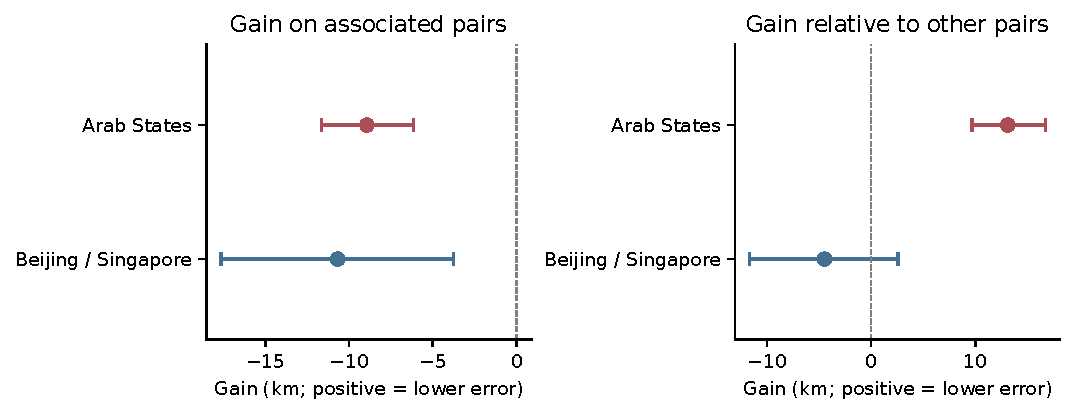
\includegraphics[width=\linewidth]{figures/local-language-effects.pdf}
\caption{Local-language gains with pointwise 95\% bootstrap intervals, conditional on repeated-call variation. These intervals do not quantify population uncertainty across cities and are not multiplicity-adjusted.}\label{fig:local}
\end{figure}


The Spanish advantage remains positive when each associated capital is omitted: home-pair gains range from 13.1 to 25.1 km and interactions from 20.3 to 32.2 km (Appendix~\ref{app:sensitivity}). French and Mandarin gains change sign under such omissions. Mandarin is particularly limited by having only two associated capitals. For comparison of estimands, median-based associated-pair gains are $-4.1$, $+23.9$, $-27.5$, and $-9.7$ km for French, Spanish, Arabic, and Mandarin respectively; their directions agree with the single-response results, but no additional tests are performed on them.

\section{Interpretation and limitations}
The observations support geographically structured, language-sensitive behavior. They do not identify independent internal maps or causal effects of linguistic culture. One translation per language confounds language with wording; the unchanged English place names further limit the intervention. Numeric-format restrictions can influence generation and may interact with language. English is a comparison condition, not a neutral view of geography.

The local-language result is conditional and exploratory. Country-language groups correlate with geography, distance range, multilingualism, and likely training-text exposure. The interaction removes a language's overall advantage on the remaining pairs; it does not adjust all these confounders. No training-corpus frequencies, city prominence measures, or population-weighted models are available in this analysis. In particular, the Spanish finding cannot be attributed causally to familiarity or cultural representation.

Repeated API calls are the unit of sampling uncertainty. Shared capitals, one model alias, one run per condition, and concurrent scheduling restrict generalization. Ten responses per pair can miss rare modes and extreme tails. A small conditional $p$ value may coexist with uncertainty about new prompts or new countries. Provider-side dependence, routing, caching, or unreported model changes would violate assumptions not verifiable from saved outputs. Symmetry has not been tested directionally, and the reported geometry depends on the aggregation rule and fitting family. No bootstrap position clouds or inferential comparisons of whole reconstructed maps were performed.

Euclidean stress must be compared with a reference-distance baseline, not interpreted as evidence that the true Earth requires extra semantic dimensions. Likewise, small spherical stress does not establish unique identification, and four numerical starts do not prove global optimality. We do not select a latent dimensionality from the scree curve. Warped country shapes depend on interpolation and fixed frame pins; only the sampled capital relationships are directly elicited.

A confirmatory extension should fix its language-affinity definition and primary estimands before collection, balance regional and distance coverage, include several independently reviewed translations per language, randomize collection blocks, and repeat on separate dates and models. Localized city-name conditions should be factorially separated from instruction language. These extensions would test whether the present Spanish-associated benefit generalizes beyond this configuration.

\section{Reproducibility and availability}
The implementation uses Python for collection and analysis and a React/Vinext frontend for exploration. CSV files store places, pairs, and append-only response attempts; JSON manifests preserve conditions and analysis parameters. There is no database. A bounded job queue, rate limiting, retries, budget accounting, per-run locking, and per-attempt flushes support resumable collection. A crash between remote completion and checkpoint writing can still repeat a billed call; the runner does not claim exactly-once provider execution.

Experiment identifiers and analysis exports are listed in the supplement. Raw responses and downstream numerical results are reproducible from saved files; future calls to a mutable provider alias need not reproduce historical behavior. The repository includes source hashes, exact prompts, analysis scripts, generated tables and figures, and this LaTeX source. The language study's recorded usage-based cost is approximately US\$9.86; this is a software estimate, not a billing invoice.

The project repository is \url{https://github.com/timini/cognitive-atlas}. It is private at the time of writing; this report does not claim public data availability or a permanent archival DOI. The hosted atlas is an access-controlled exploration interface. Running the paper analysis and build requires no API key and makes no model calls. Author identities, affiliations, and submission metadata are intentionally not assigned in this research draft. Code, analysis, translations, and drafting were prepared with AI assistance; human scientific and language review remains necessary before submission.

\section{Conclusion}
Repeated pairwise judgments make it possible to reconstruct and audit the geography expressed by a language model while preserving response variation. In the matched Gemini 3.5 Flash runs, all instruction languages change the distance matrix detectably under a conditional permutation baseline, even when aggregate accuracy remains similar. A separate exploratory analysis finds an accuracy benefit for Spanish-associated capitals under Spanish instructions, but no general local-language advantage. The evidence concerns elicited geographic behavior on a fixed benchmark; broader claims require replication across prompts, places, dates, and models.

\bibliographystyle{plain}
\bibliography{references}

\clearpage
\appendix
\section{All language comparisons}\label{app:comparisons}

\begin{table}[htbp]\centering\small
\caption{Complete-pair median statistics. Disagreement is $T_{ab}$. MAE change is second minus first language; positive means the second is worse. Both $p$ columns are Holm-adjusted across twenty tests under the strong exchangeability null.}\label{tab:pairwise}
\begin{tabular}{lrrrr}\toprule
First / second & Disagreement (km) & MAE change (km) & $p_T$ & $p_A$ \\\midrule
\tableinput{generated/pairwise-table.tex}
\bottomrule\end{tabular}
\end{table}

The complete-case median-based MAEs are 164.5 km (English), 156.9 km (French), 166.5 km (Spanish), 185.4 km (Arabic), and 165.2 km (Mandarin). These differ slightly from Table~\ref{tab:languages}, which includes all pairs with their available valid responses. The exclusion rule is identical for all comparisons; it is not chosen separately to maximize a result.

\section{Capital omission sensitivity}\label{app:sensitivity}

\begin{table}[htbp]\centering\small
\caption{Descriptive ranges after removing one language-associated capital and all its pairs. Positive values favor the translated prompt. These are sensitivity ranges, not confidence intervals.}
\begin{tabular}{lrr}\toprule
Language & Associated-pair gain range (km) & Interaction range (km) \\\midrule
\tableinput{generated/leaveout-table.tex}
\bottomrule\end{tabular}
\end{table}

The full supplement identifies the omitted capital for each estimate. Removing Dakar changes the French associated-pair gain from negative to positive. Removing Beijing leaves a positive Mandarin gain for Singapore-associated pairs; removing Singapore leaves a negative gain for Beijing-associated pairs. A single group summary therefore conceals meaningful city heterogeneity.

\clearpage
\section{Protocol and experiment identifiers}
The English numeric protocol is reproduced below; the machine-readable supplement contains the exact Unicode versions of all five prompts and the manifests contain the parameter values.
\begin{quote}\small
Estimate the straight-line great-circle distance in kilometres between \{city\_a\}, \{country\_a\} and \{city\_b\}, \{country\_b\}. Return only your best numerical estimate in kilometres. Do not explain your reasoning. Use only digits 0--9, with a period if a decimal separator is needed. Do not include thousands separators or units.
\end{quote}
The rendered dash above is typographic; the JSON supplement preserves the exact prompt bytes. The language-family identifier is \texttt{great-circle-formatted-number-v2}; the parser is \texttt{ascii\_decimal\_v2}. The 50-capital dataset SHA-256 is
\begin{center}\scriptsize\texttt{835b87cc327926b228c86d1e17cfe797c903497661a1603843d7f7662f62ef9e}\end{center}

\begin{table}[htbp]\centering\small
\caption{Immutable experiment identifiers, including the earlier 20-capital pilot. Full export identifiers and result hashes are in \texttt{results/provenance.json}.}
\begin{tabular}{llrl}\toprule
Gemini configuration & Language & Capitals & Experiment ID \\\midrule
\tableinput{generated/experiments-table.tex}
\bottomrule\end{tabular}
\end{table}


\clearpage
\section{Complete capital sample}\label{app:capitals}
\small
\begin{longtable}{llp{8cm}}
\toprule ISO & Capital & Country \\\midrule\endfirsthead
\toprule ISO & Capital & Country \\\midrule\endhead
\bottomrule\endfoot
\tableinput{generated/capitals-table.tex}
\end{longtable}
\end{document}
